\subsubsection{Scope}

\begin{figure}[H]
	\centering
	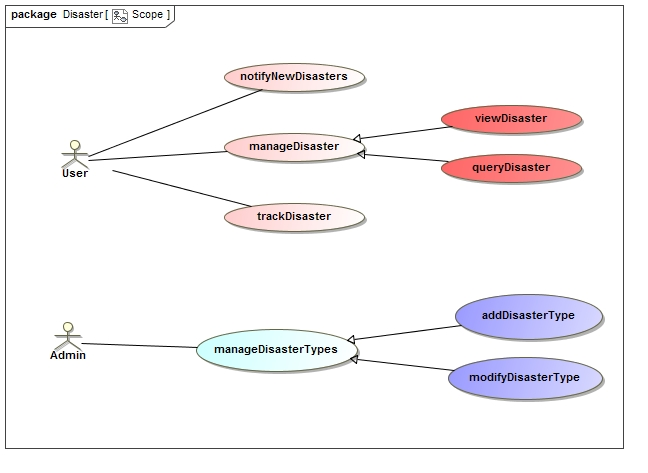
\includegraphics[scale=0.77]{../images/funcReq/DisasterScope.jpg}
	\caption{The scope of functionality required from the disaster module \label{overflow}}
\end{figure}

Admin can add and/or modify the different kinds of disaster types that are required whilst users are able to track and manage disasters as well as get notifications for new disasters. 

\subsubsection{viewDisaster}

A user can view disasters by going on to the disasters tab on the system and viewing all the disasters, active or not, that are occurring throughout the world. Below are the service contract, activity diagram and functional requirements diagram for viewDisaster.

\begin{figure}[H]
	\centering
	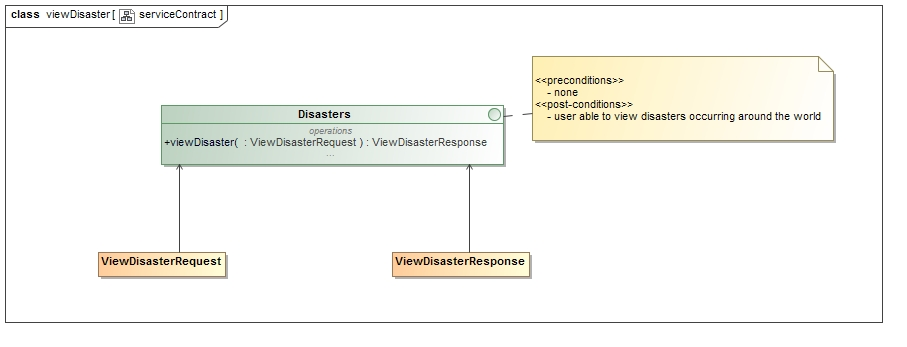
\includegraphics[scale=0.19]{../images/funcReq/viewDisasterServiceContract.jpg} 
	\caption{The service contract for viewDisaster \label{overflow}}
\end{figure}

\begin{figure}[H]
	\centering
	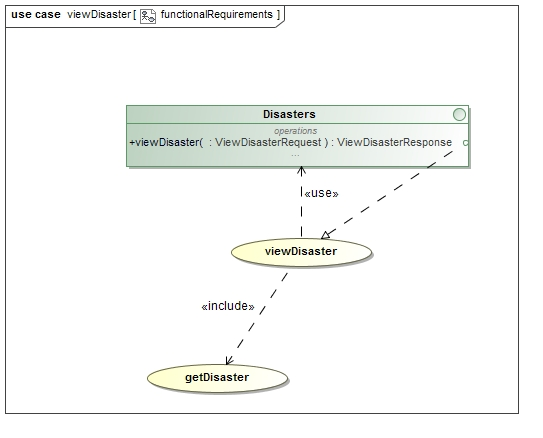
\includegraphics[width=1.2\textwidth]{../images/funcReq/viewDisasterFunctionalRequirements.jpg}
	\caption{The functional requirements diagram for viewDisaster \label{overflow}}
\end{figure}

\begin{figure}[H]
	\centering
	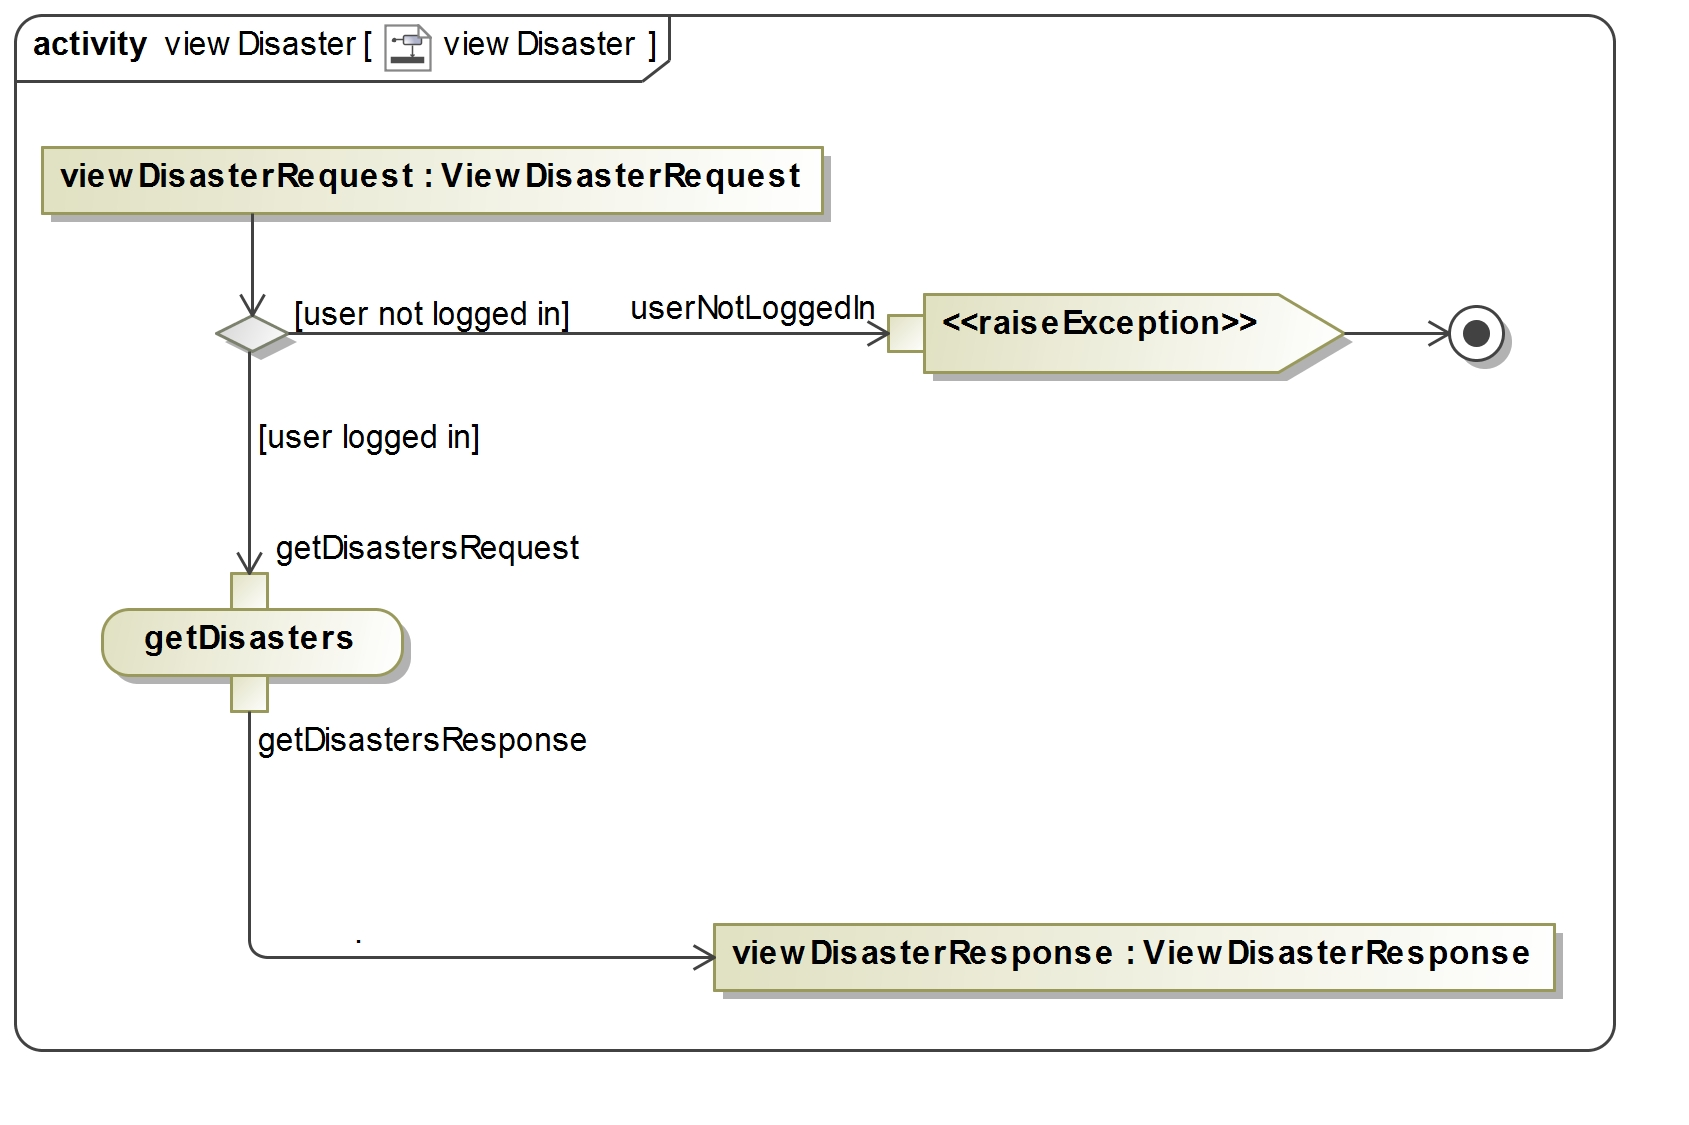
\includegraphics[width=1.2\textwidth]{../images/funcReq/viewDisasterActivityDiagram.jpg}
	\caption{The activity diagram for viewDisaster \label{overflow}}
\end{figure}

\subsubsection{queryDisaster}

The user will be able to query the system for specific disasters, by entering search criteria, such as a start date and/or a end date, so that only disasters matching the specified criteria are returned to the user. Below are the service contract, activity diagram and functional requirements diagram for queryDisaster.

 \begin{figure}[H]
	\centering
	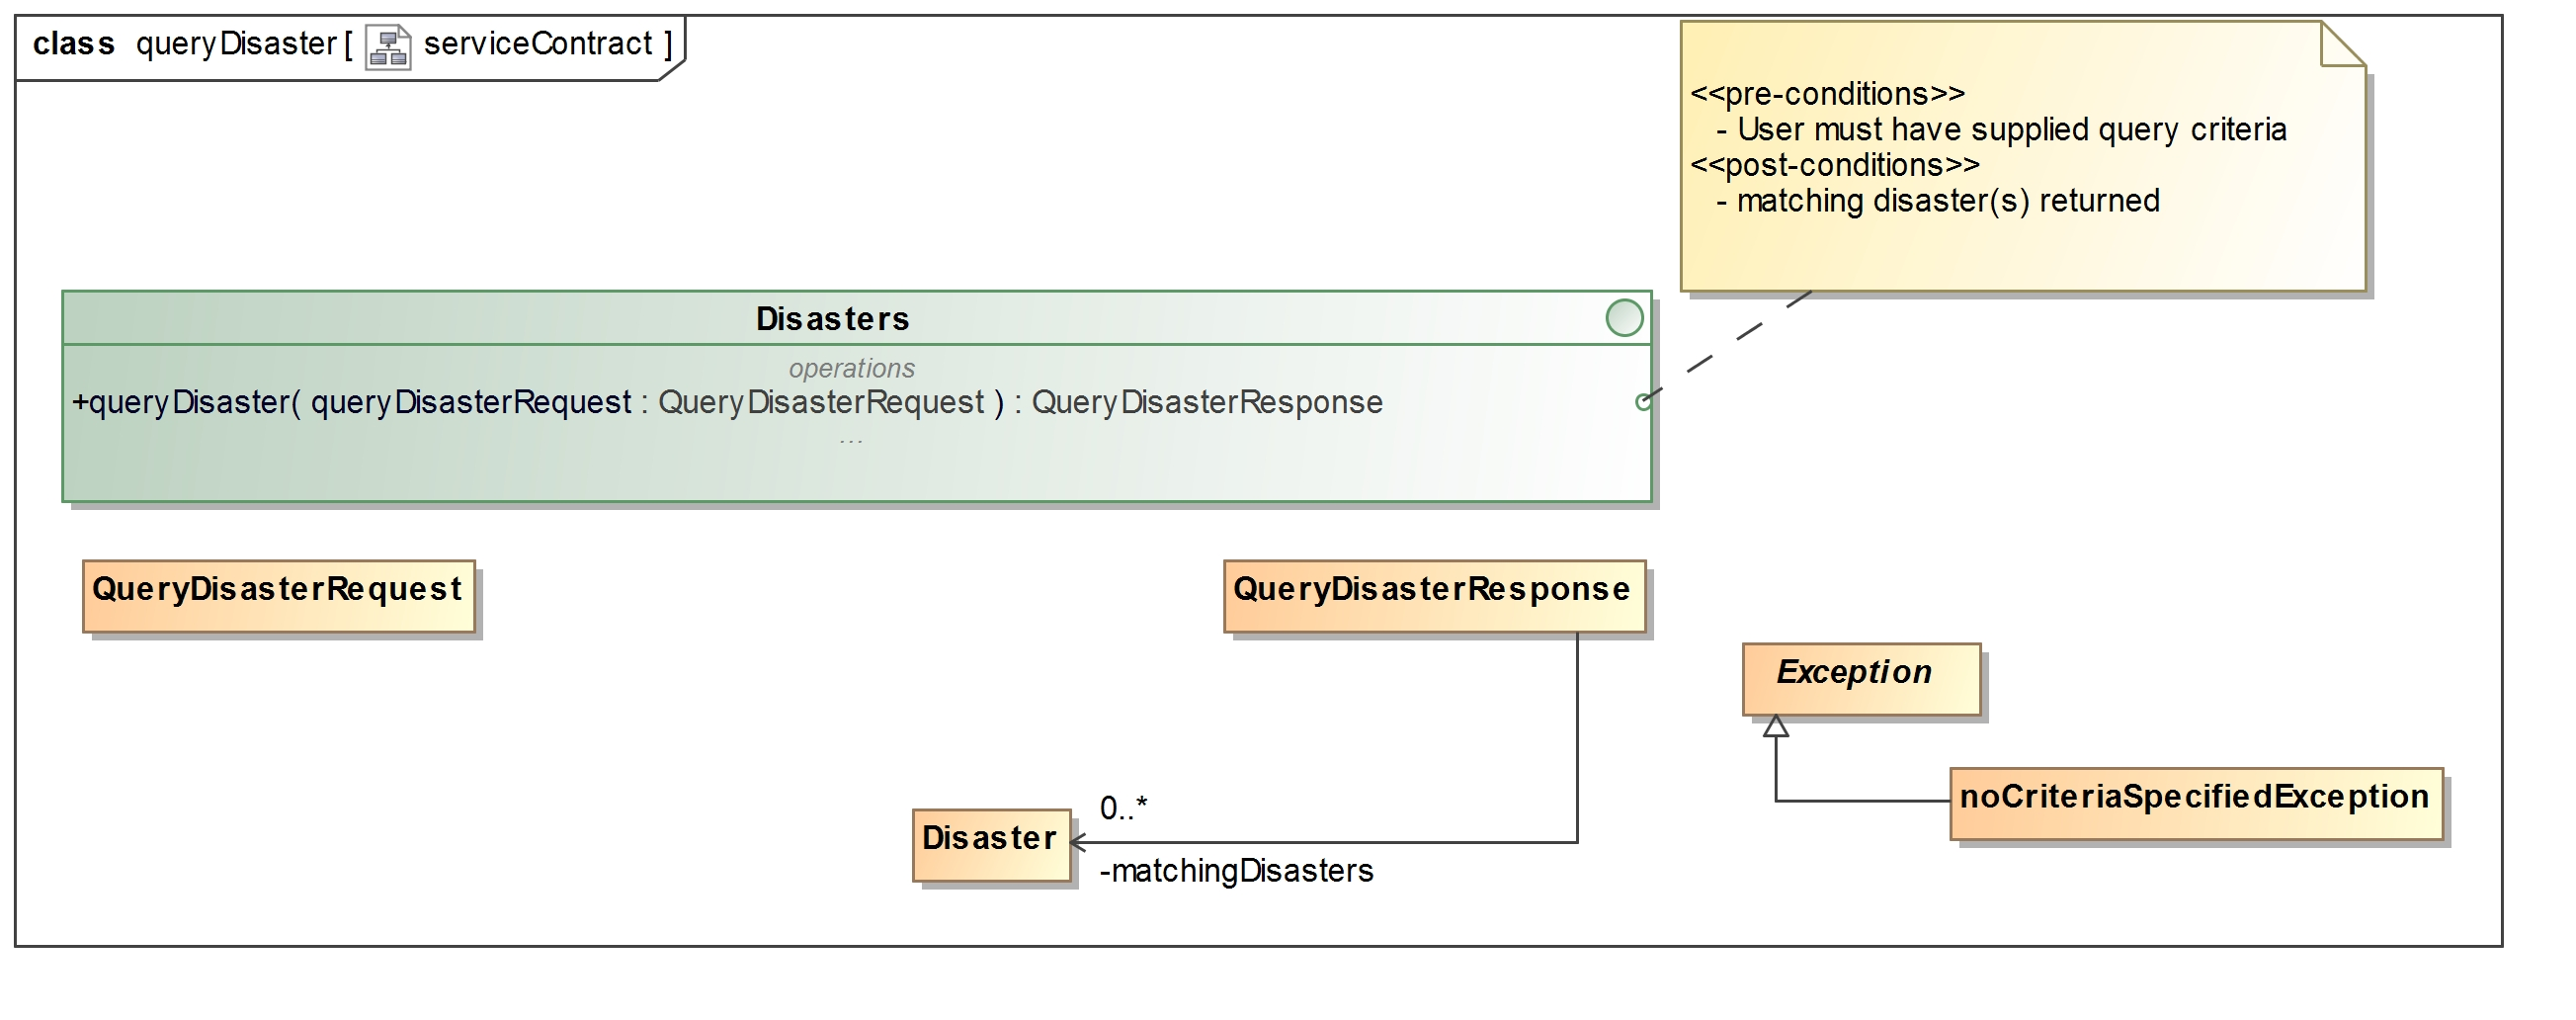
\includegraphics[scale=0.19]{../images/funcReq/queryDisasterServiceContract.jpg}
	\caption{The service contract for queryDisaster \label{overflow}}
\end{figure}

\begin{figure}[H]
	\centering
	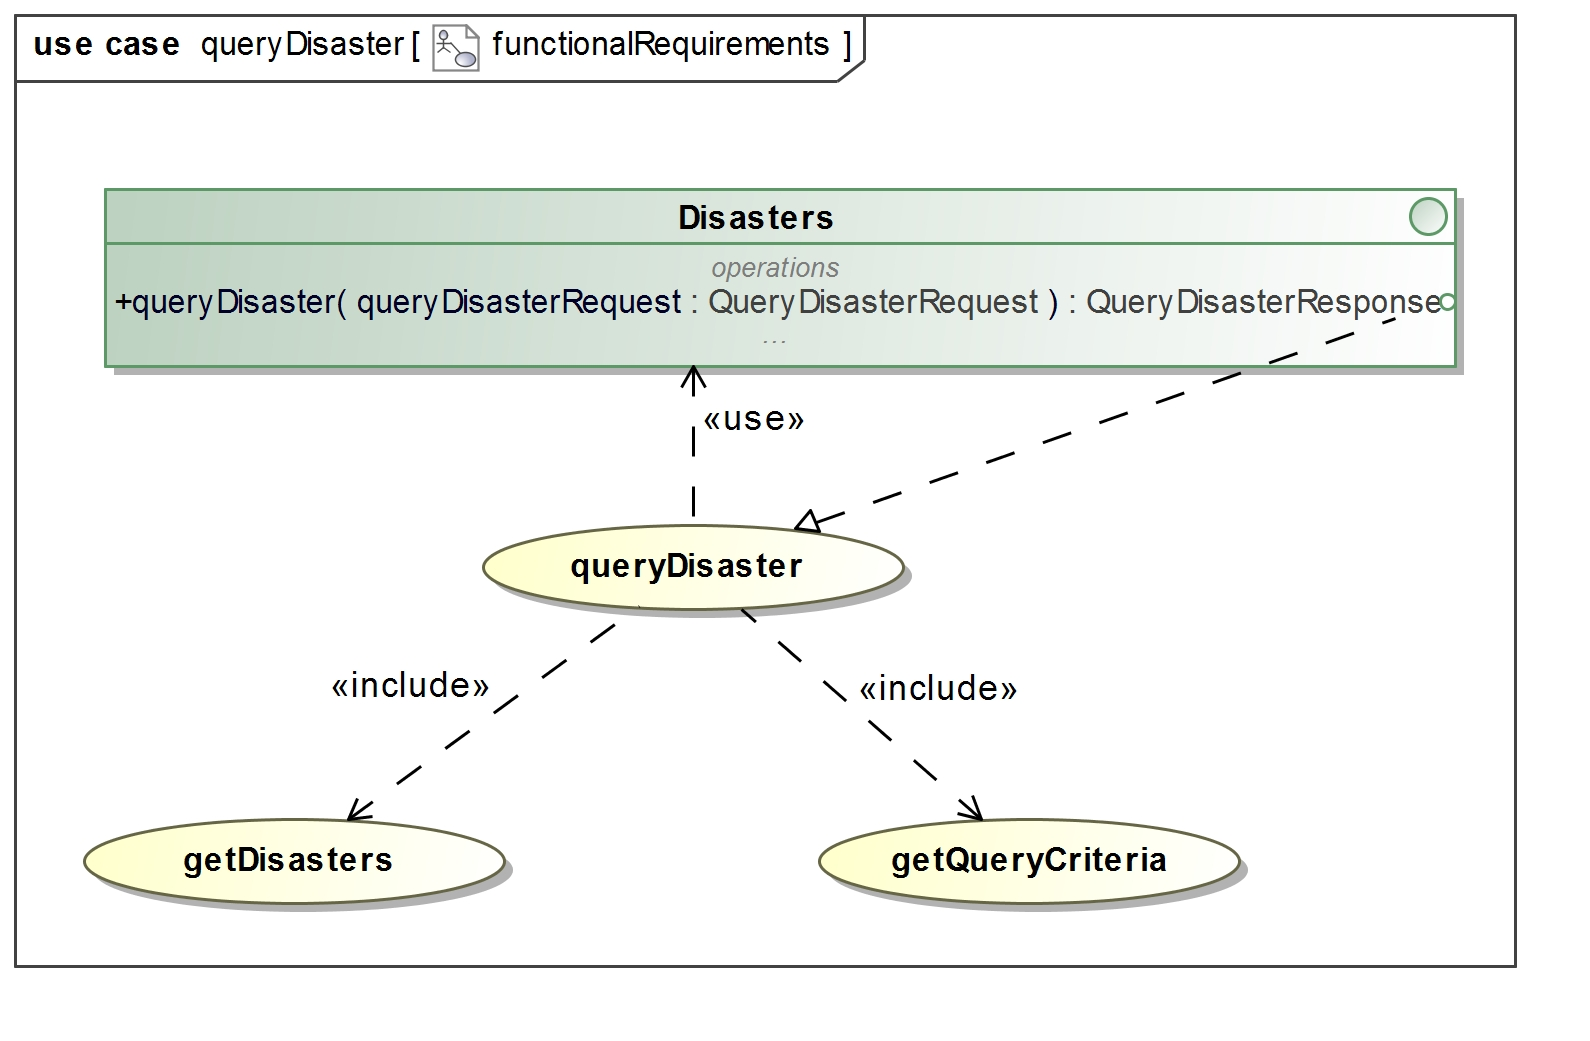
\includegraphics[width=1.2\textwidth]{../images/funcReq/queryDisasterFunctionalRequirements.jpg}
	\caption{The functional requirements diagram for queryDisaster \label{overflow}}
\end{figure}

\begin{figure}[H]
	\centering
	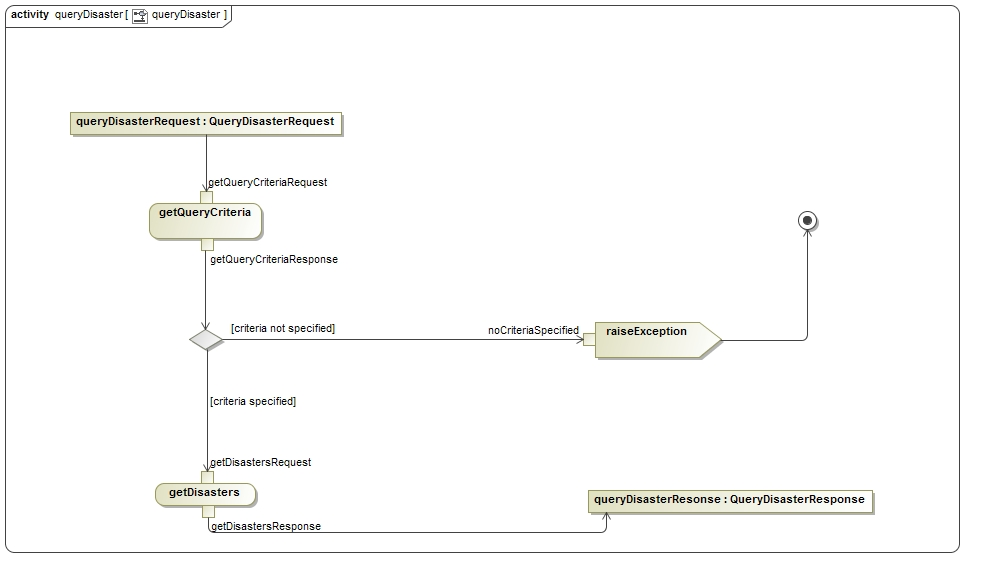
\includegraphics[scale=0.2]{../images/funcReq/queryDisasterActivityDiagram.jpg}
	\caption{The activity diagram for queryDisaster \label{overflow}}
\end{figure} 

\subsubsection{notifyNewDisaster}

A user will be able to be notified of any new disasters that are occuring as of the time they are using the system as long as that disaster is not visualized on the system yet. Below are the service contract, activity diagram and functional requirements diagram for notifyNewDisaster.

 \begin{figure}[H]
	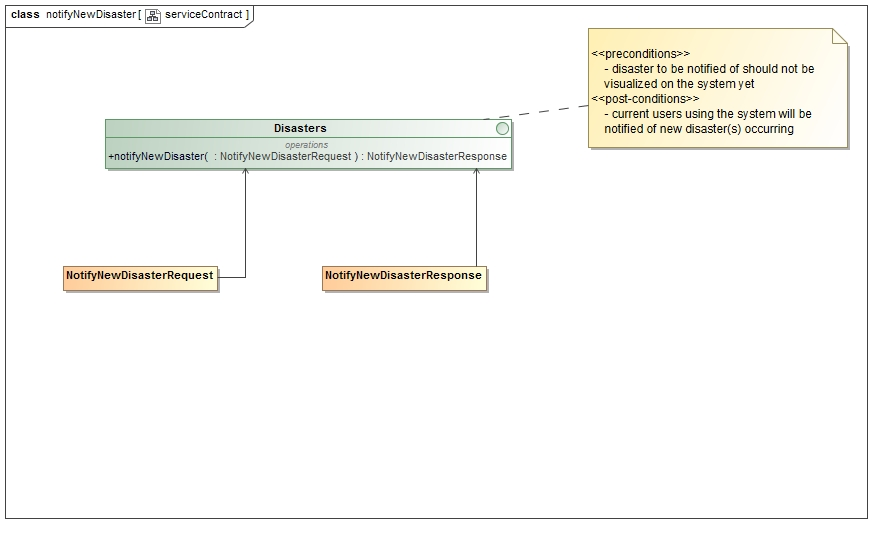
\includegraphics[scale=0.2]{../images/funcReq/notifyNewDisasterServiceContract.jpg}
	\caption{The service contract for notifyNewDisaster \label{overflow}}
\end{figure}

\begin{figure}[H]
	\centering
	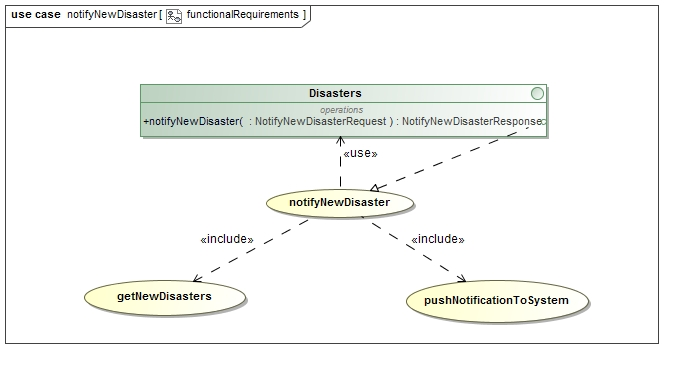
\includegraphics[width=1.2\textwidth]{../images/funcReq/notifyNewDisasterFunctionalRequirements.jpg}
	\caption{The functional requirements diagram for notifyNewDisaster \label{overflow}}
\end{figure}

\begin{figure}[H]
	\centering
	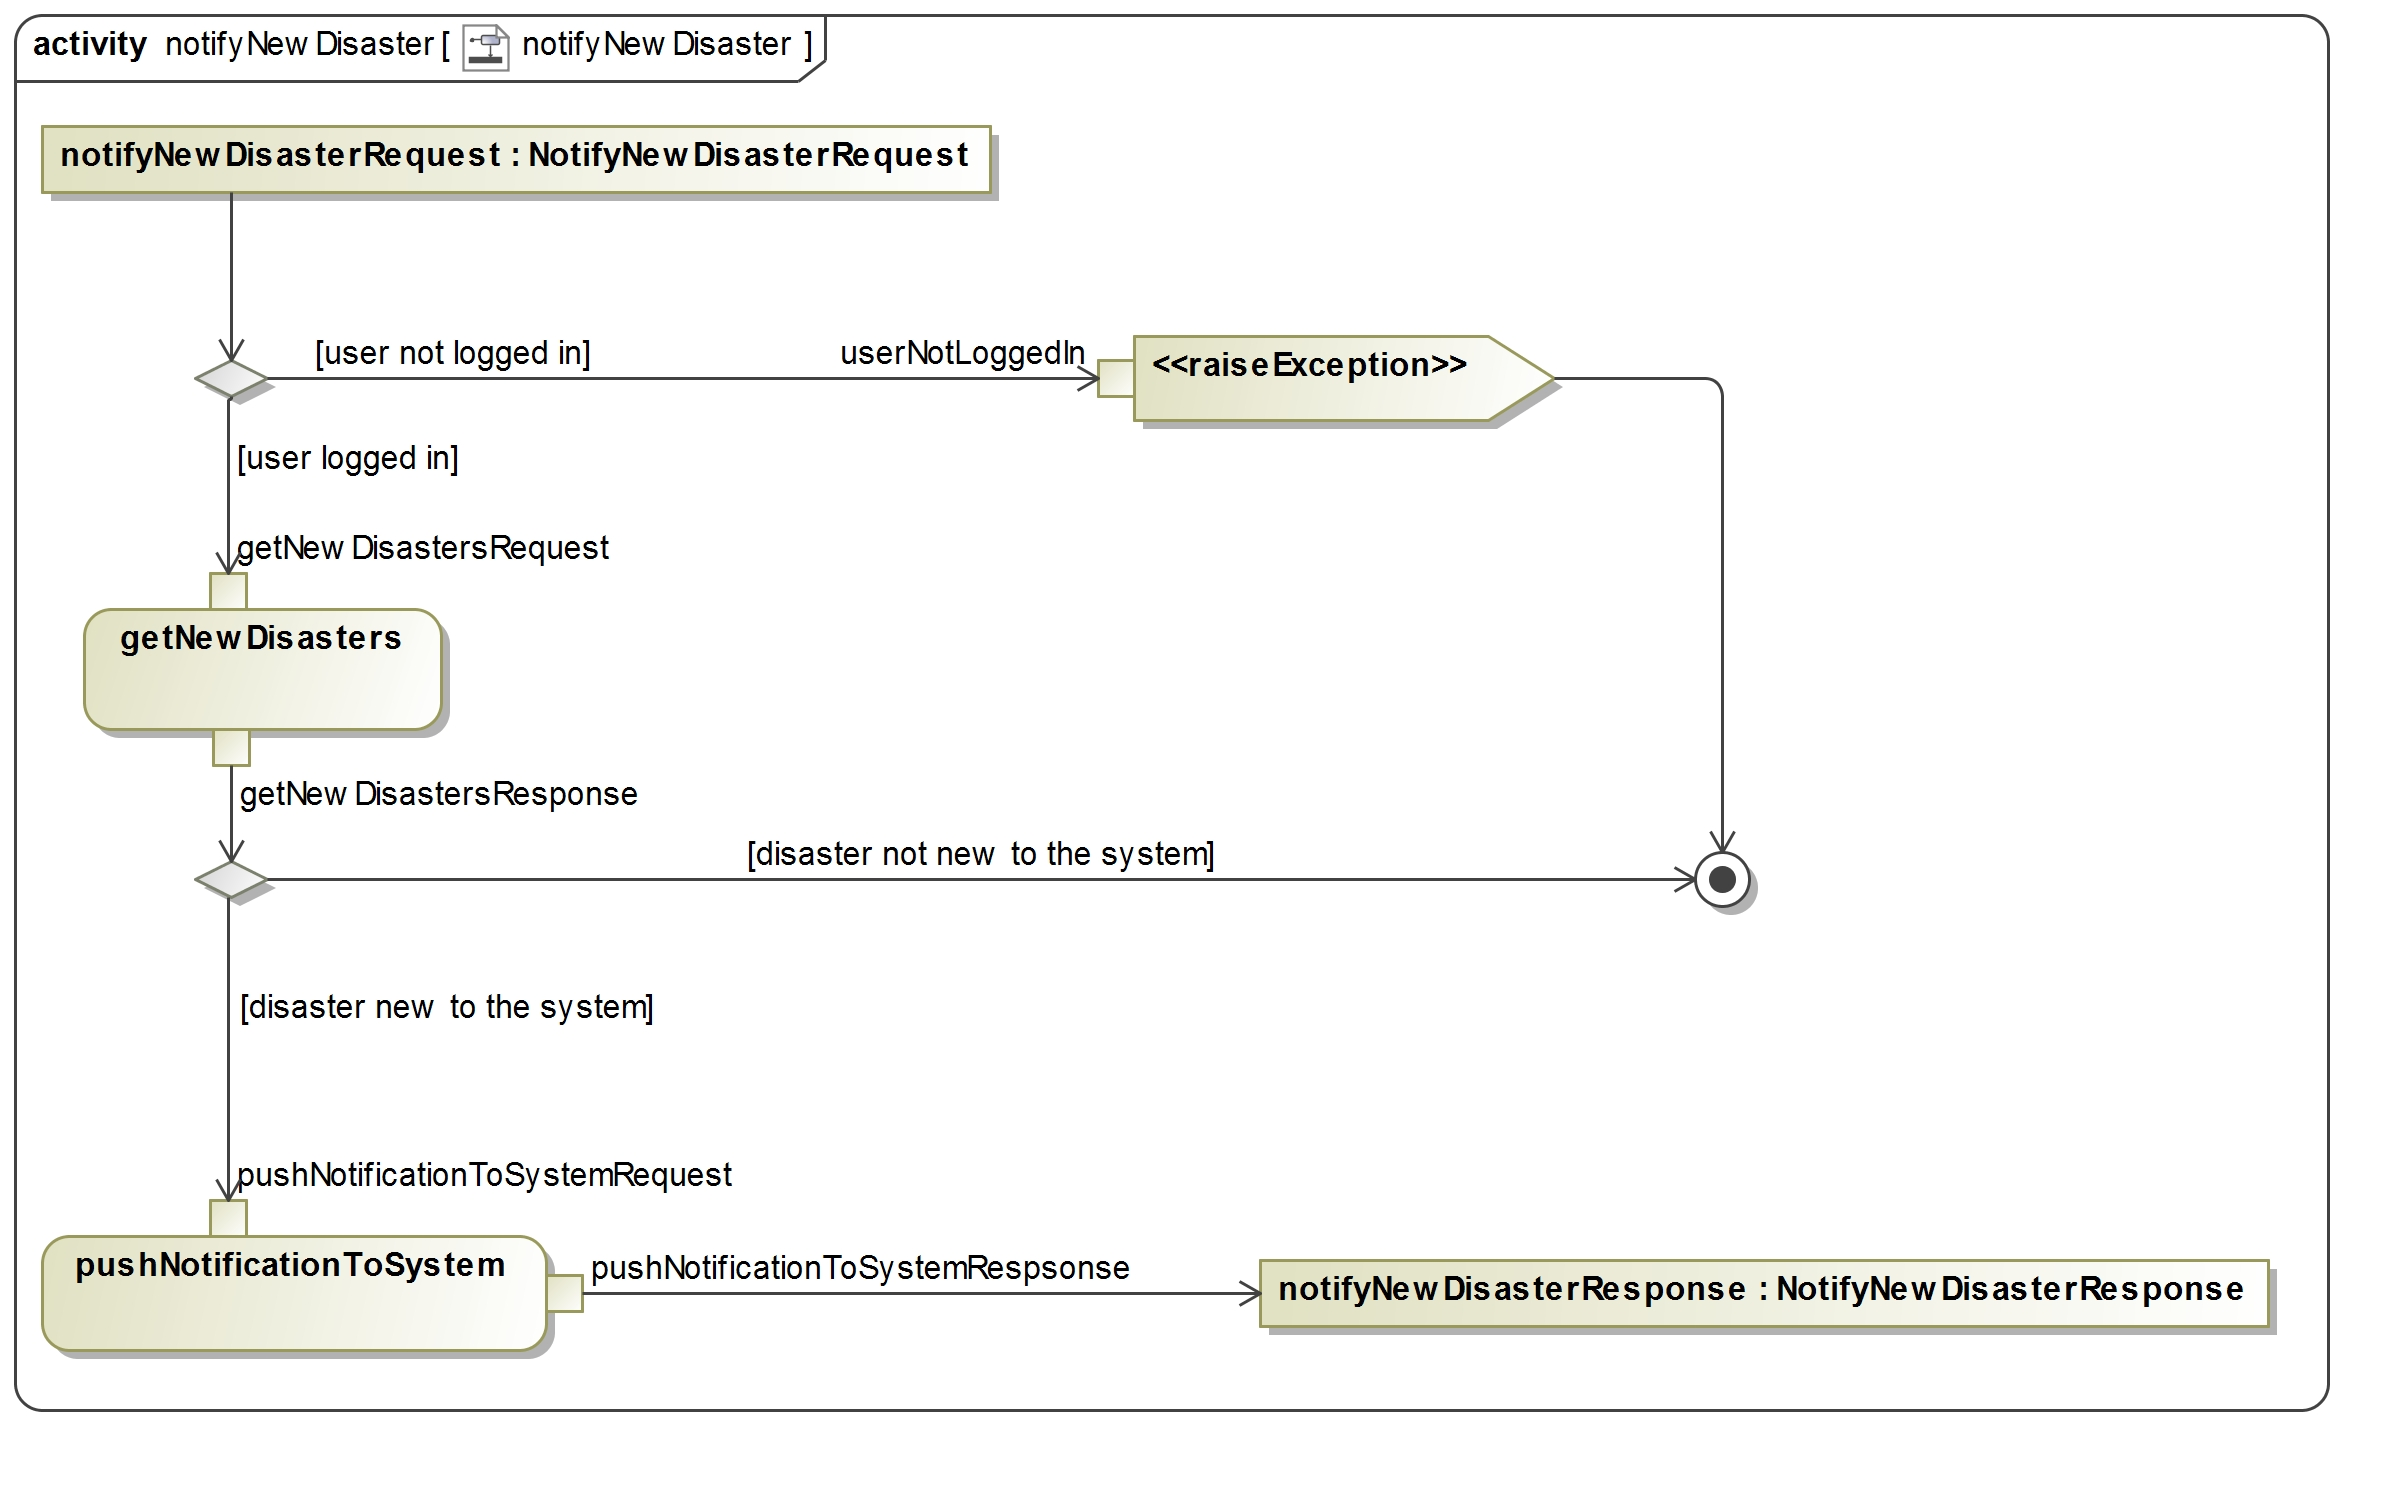
\includegraphics[scale=0.22]{../images/funcReq/notifyNewDisasterActivityDiagram.jpg}
	\caption{The activity diagram for notifyNewDisaster \label{overflow}}
\end{figure} 

\subsubsection{trackDisaster}

A user is able to track a disaster as long as the disaster is still active and data for the disaster is updated regurlarly. Below are the service contract, activity diagram and functional requirements diagram for trackDisaster.

\begin{figure}[H]
	\centering
	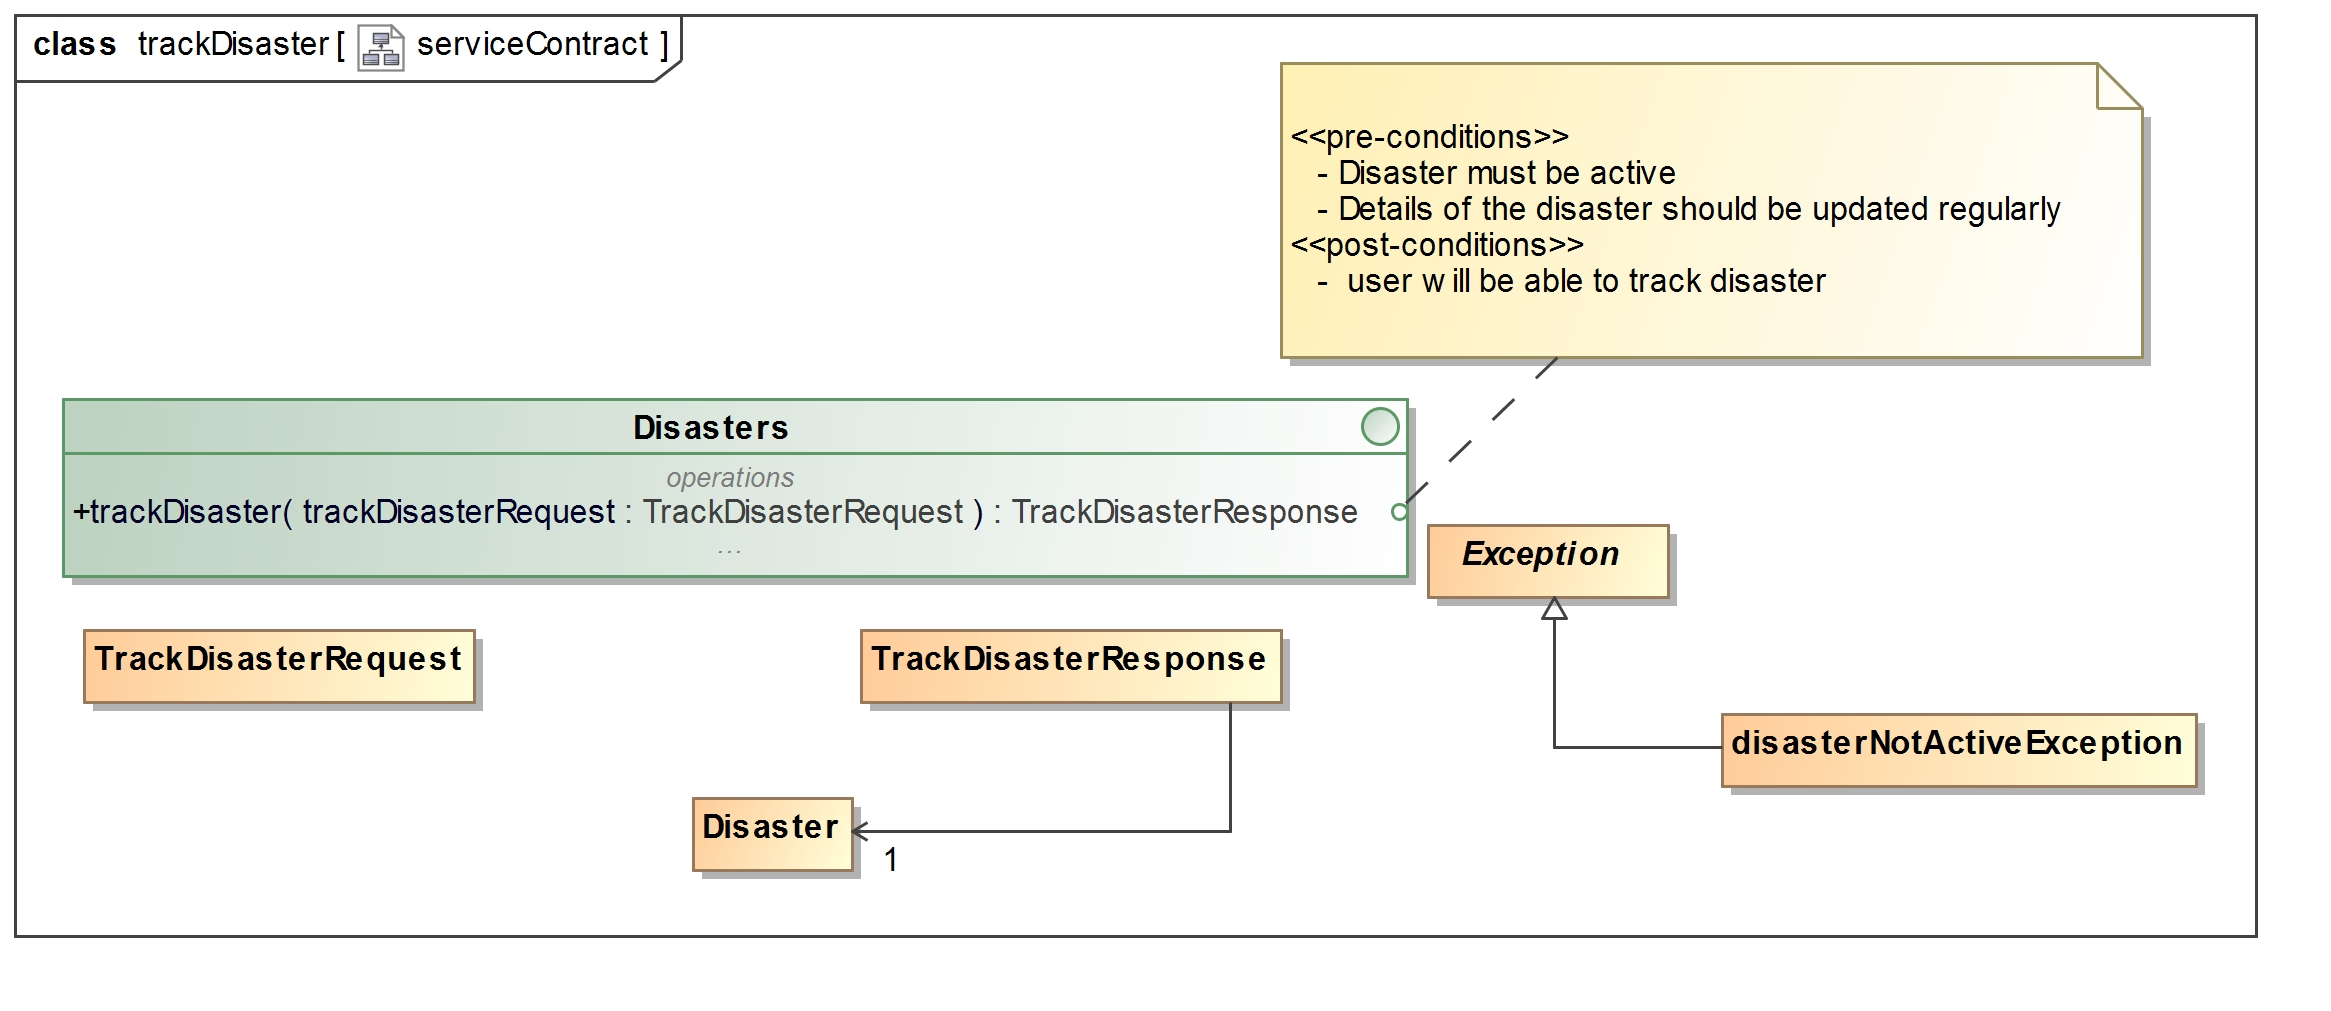
\includegraphics[scale=0.21]{../images/funcReq/trackDisasterServiceContract.jpg}
	\caption{The service contract for trackDisaster \label{overflow}}
\end{figure}

\begin{figure}[H]
	\centering
	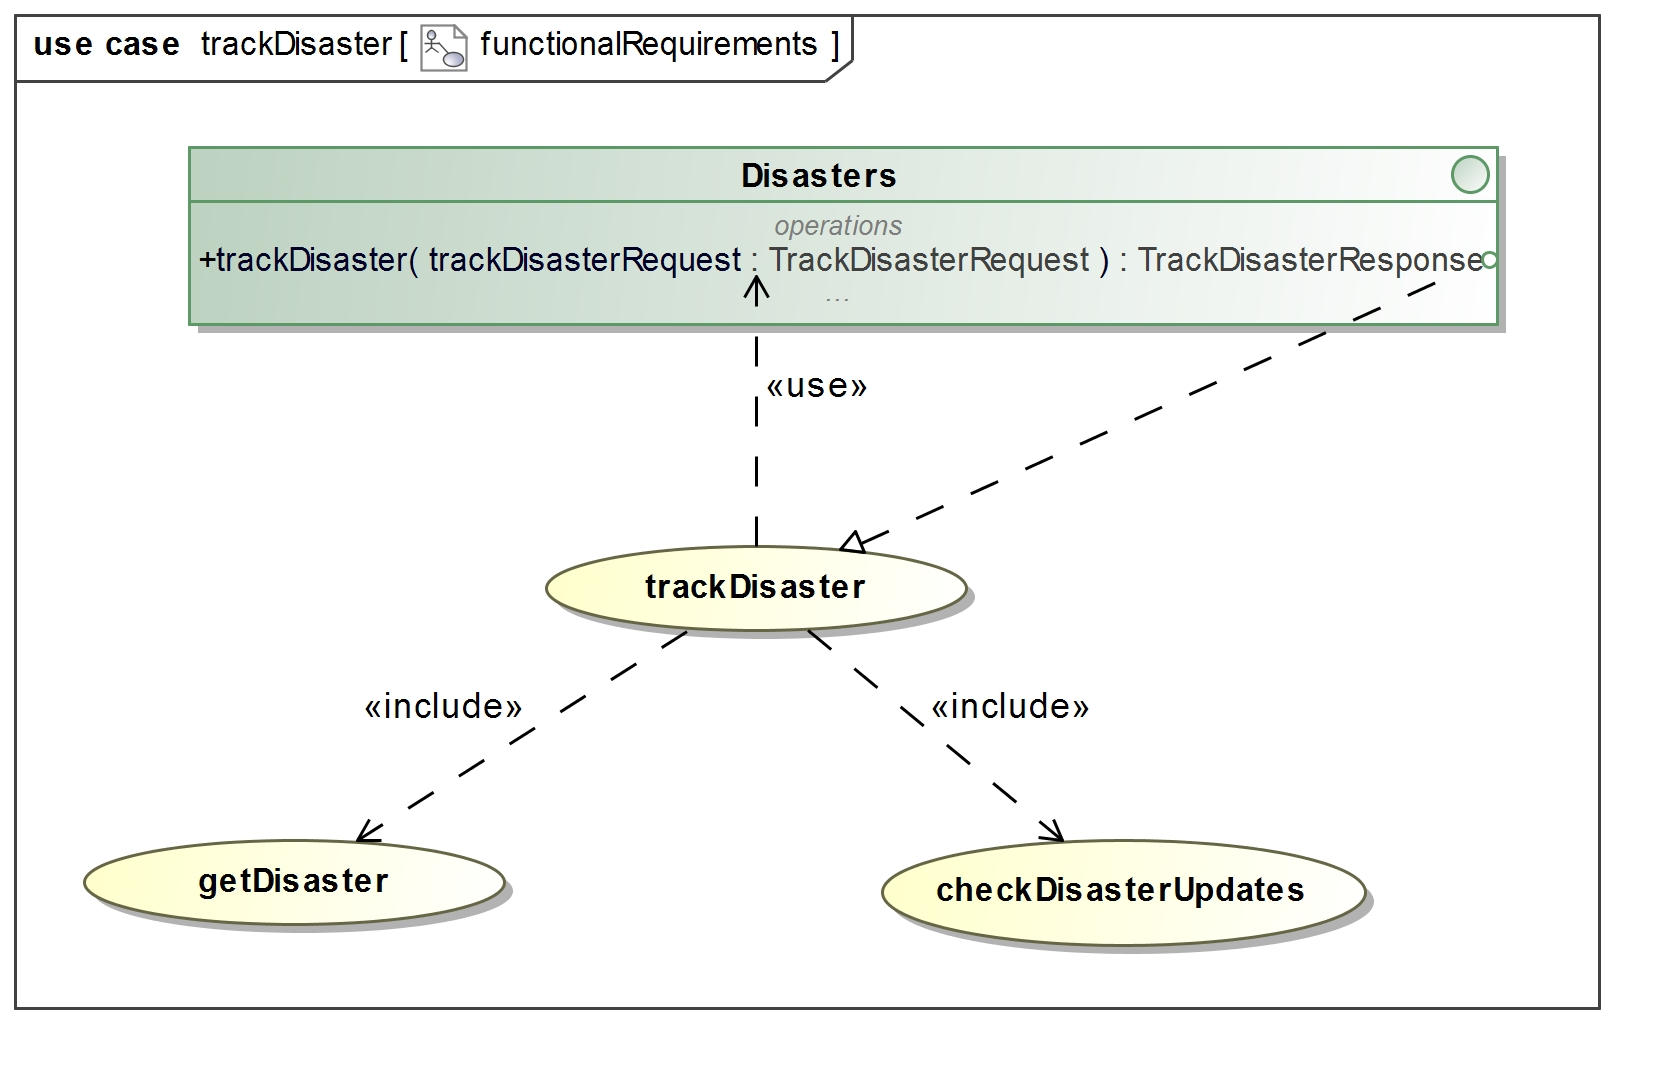
\includegraphics[width=1.2\textwidth]{../images/funcReq/trackDisasterFunctionalRequirements.jpg}
	\caption{The functional requirements diagram for trackDisaster \label{overflow}}
\end{figure}

\begin{figure}[H]
	\centering
	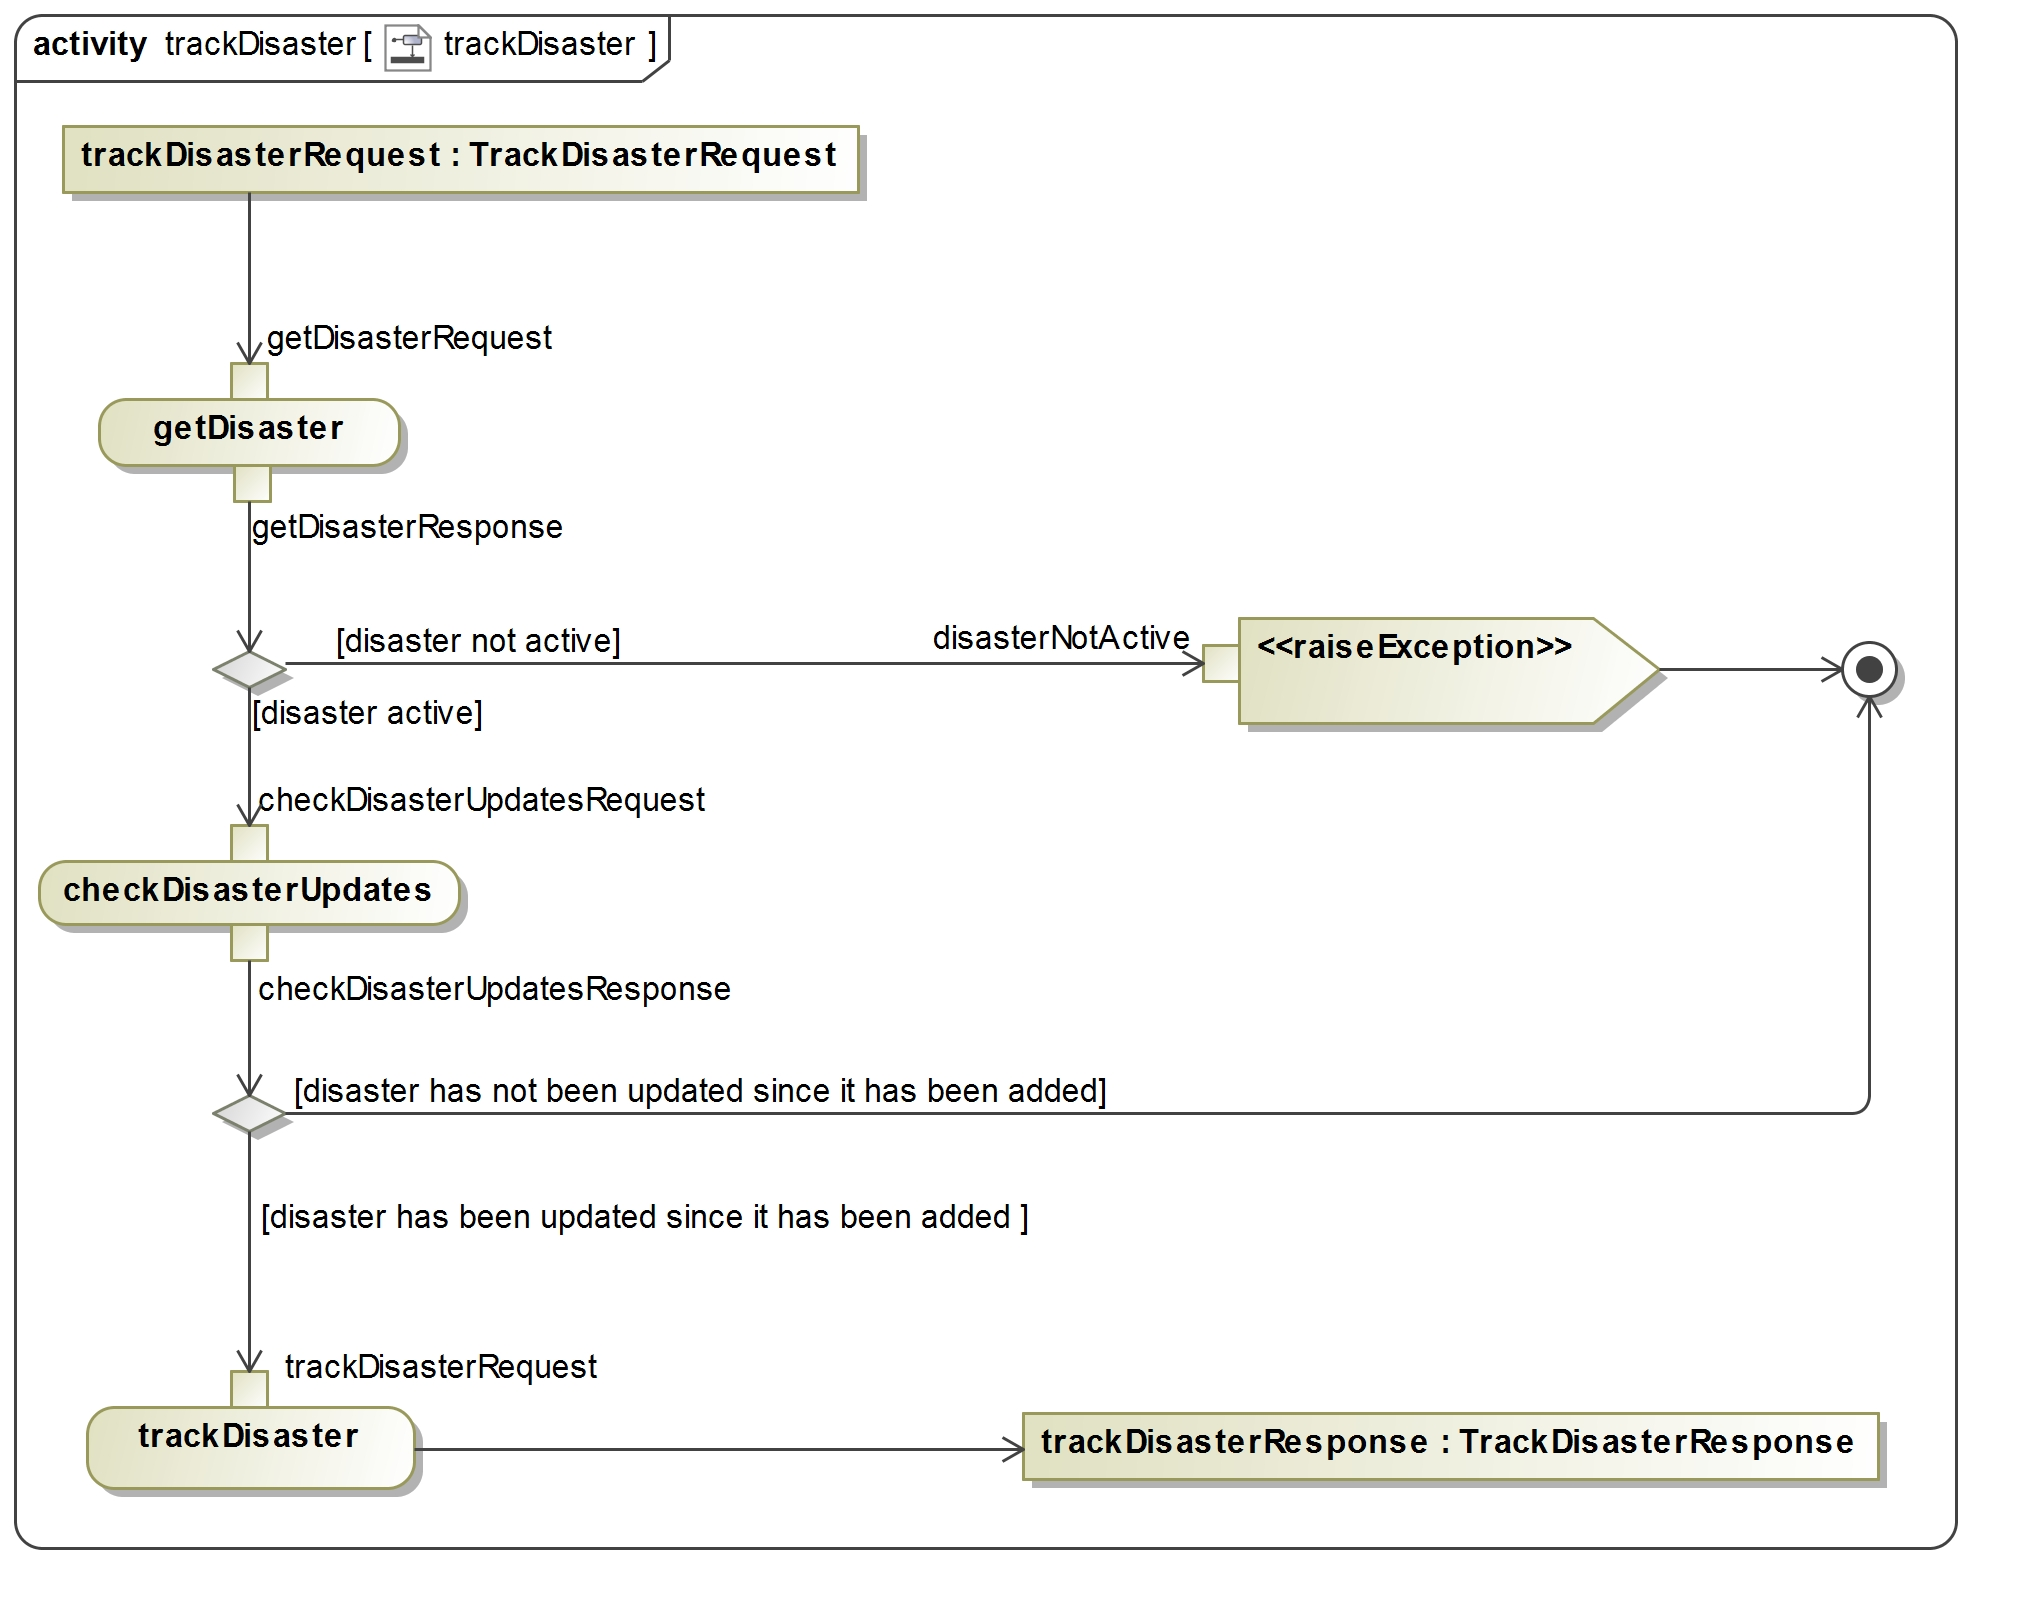
\includegraphics[width=1.2\textwidth]{../images/funcReq/trackDisasterActivityDiagram.jpg}
	\caption{The activity diagram for trackDisaster \label{overflow}}
\end{figure}

\subsubsection{addDisasterType}

Adding a disaster type requires that the user has admin rights and that there should not be a disaster type of the type being added that exists. If the user is admin and the disaster type being added is unique then a new disaster type will be added to the system. Below are the service contract, activity diagram and functional requirements diagram for addDisasterType.

\begin{figure}[H]
	\centering
	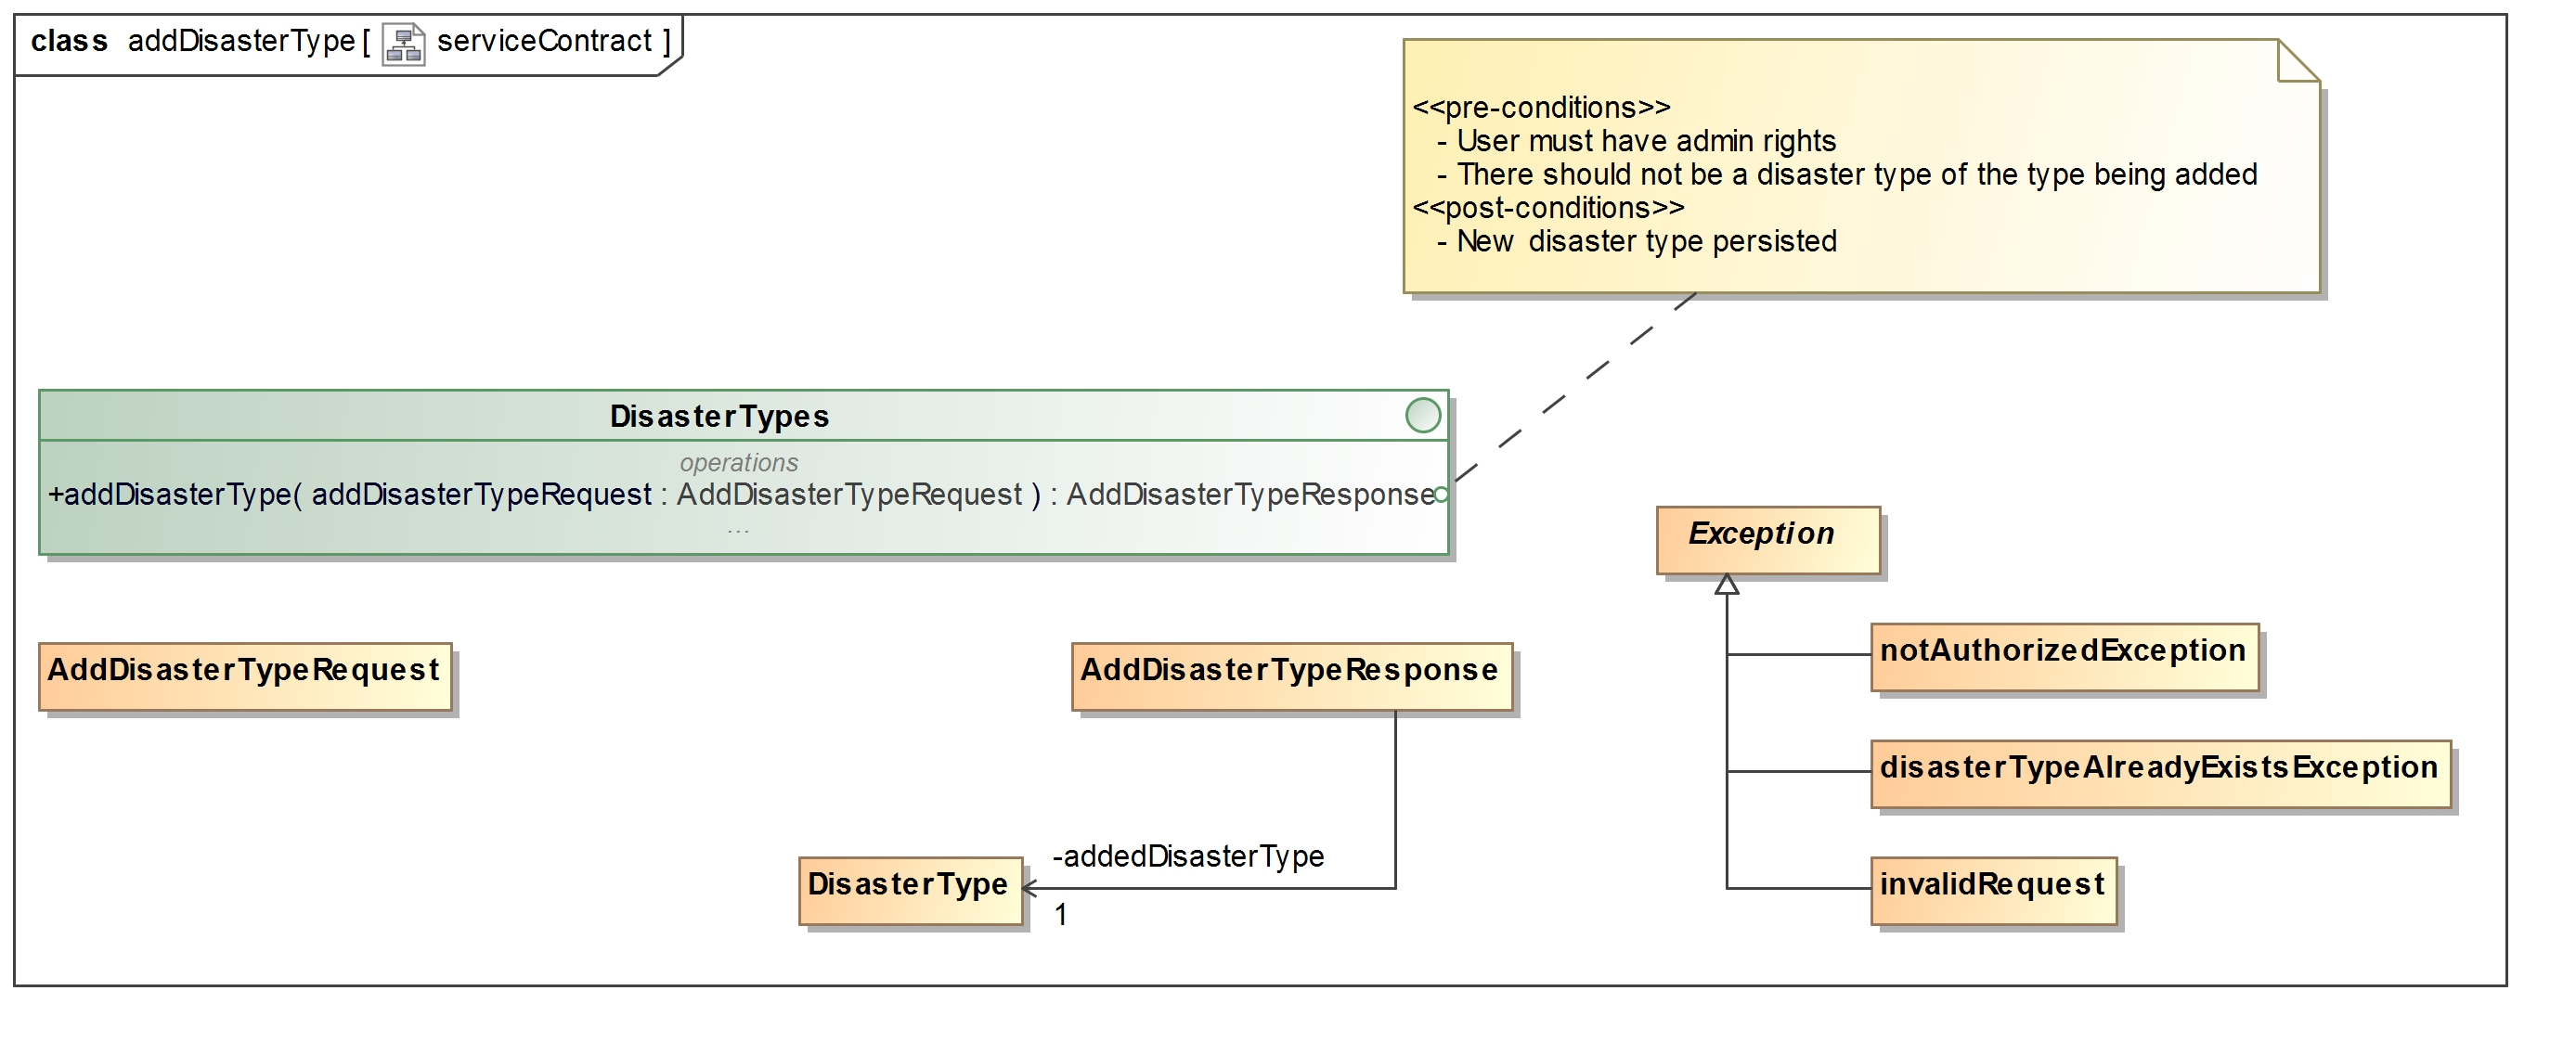
\includegraphics[scale=0.18]{../images/funcReq/addDisasterTypeServiceContract.jpg}
	\caption{The service contract for addDisasterType \label{overflow}}
\end{figure}

\begin{figure}[H]
	\centering
	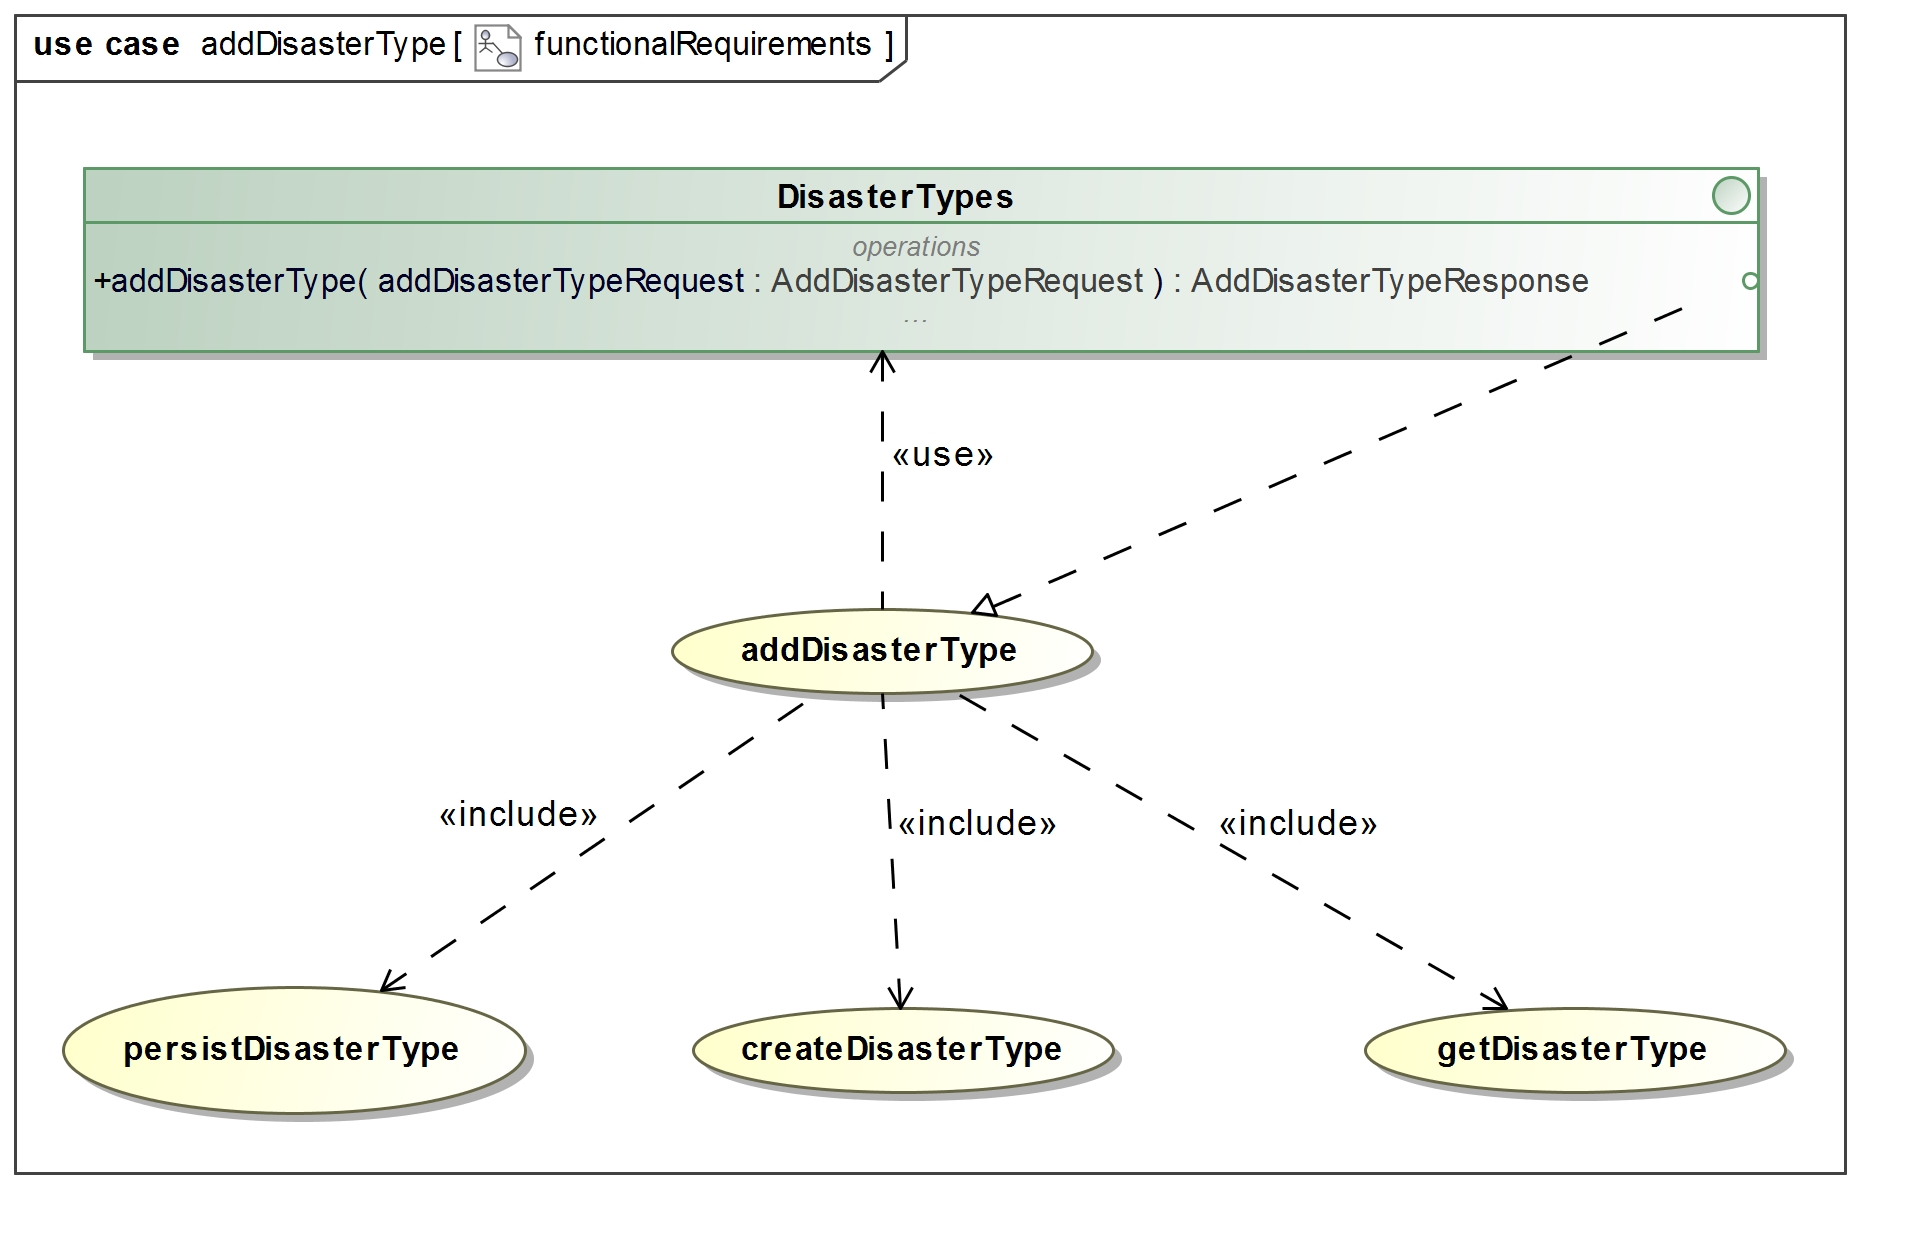
\includegraphics[width=1.2\textwidth]{../images/funcReq/AddDisasterTypeFunctionalRequirements.jpg}
	\caption{The functional requirements diagram for addDisasterType \label{overflow}}
\end{figure}

\begin{figure}[H]
	\centering
	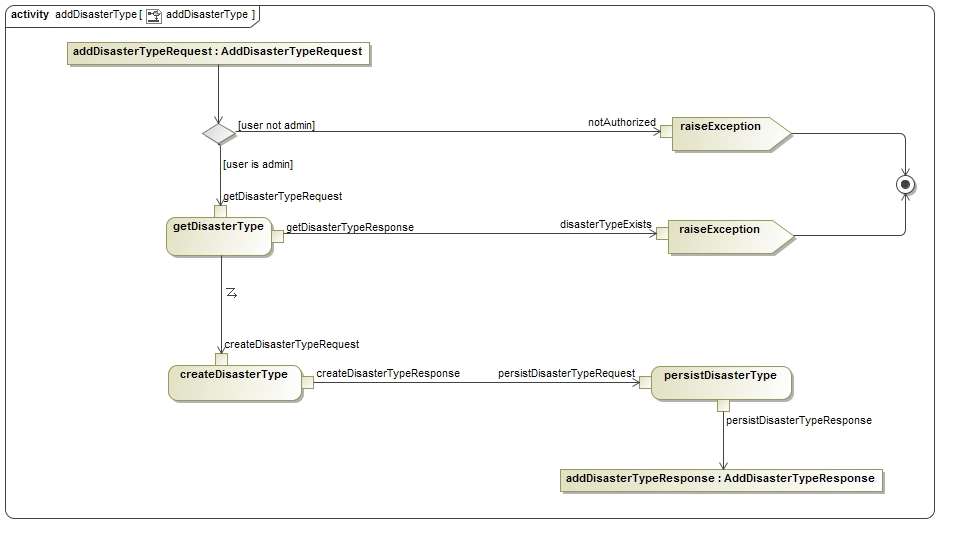
\includegraphics[scale=0.22]{../images/funcReq/addDisasterTypeActivityDiagram.jpg}
	\caption{The activity diagram for addDisasterType \label{overflow}}
\end{figure}

\subsubsection{modifyDisasterType}

Modifying a disaster type requires that the user has admin rights and that there should not be a disaster type of the same type as the modified one. If the user is admin and the modified disaster type is unique then the modified disaster type will be persisted to the database. Below are the service contract, activity diagram and functional requirements diagram for modifiyDisasterType.

\begin{figure}[H]
	\centering
	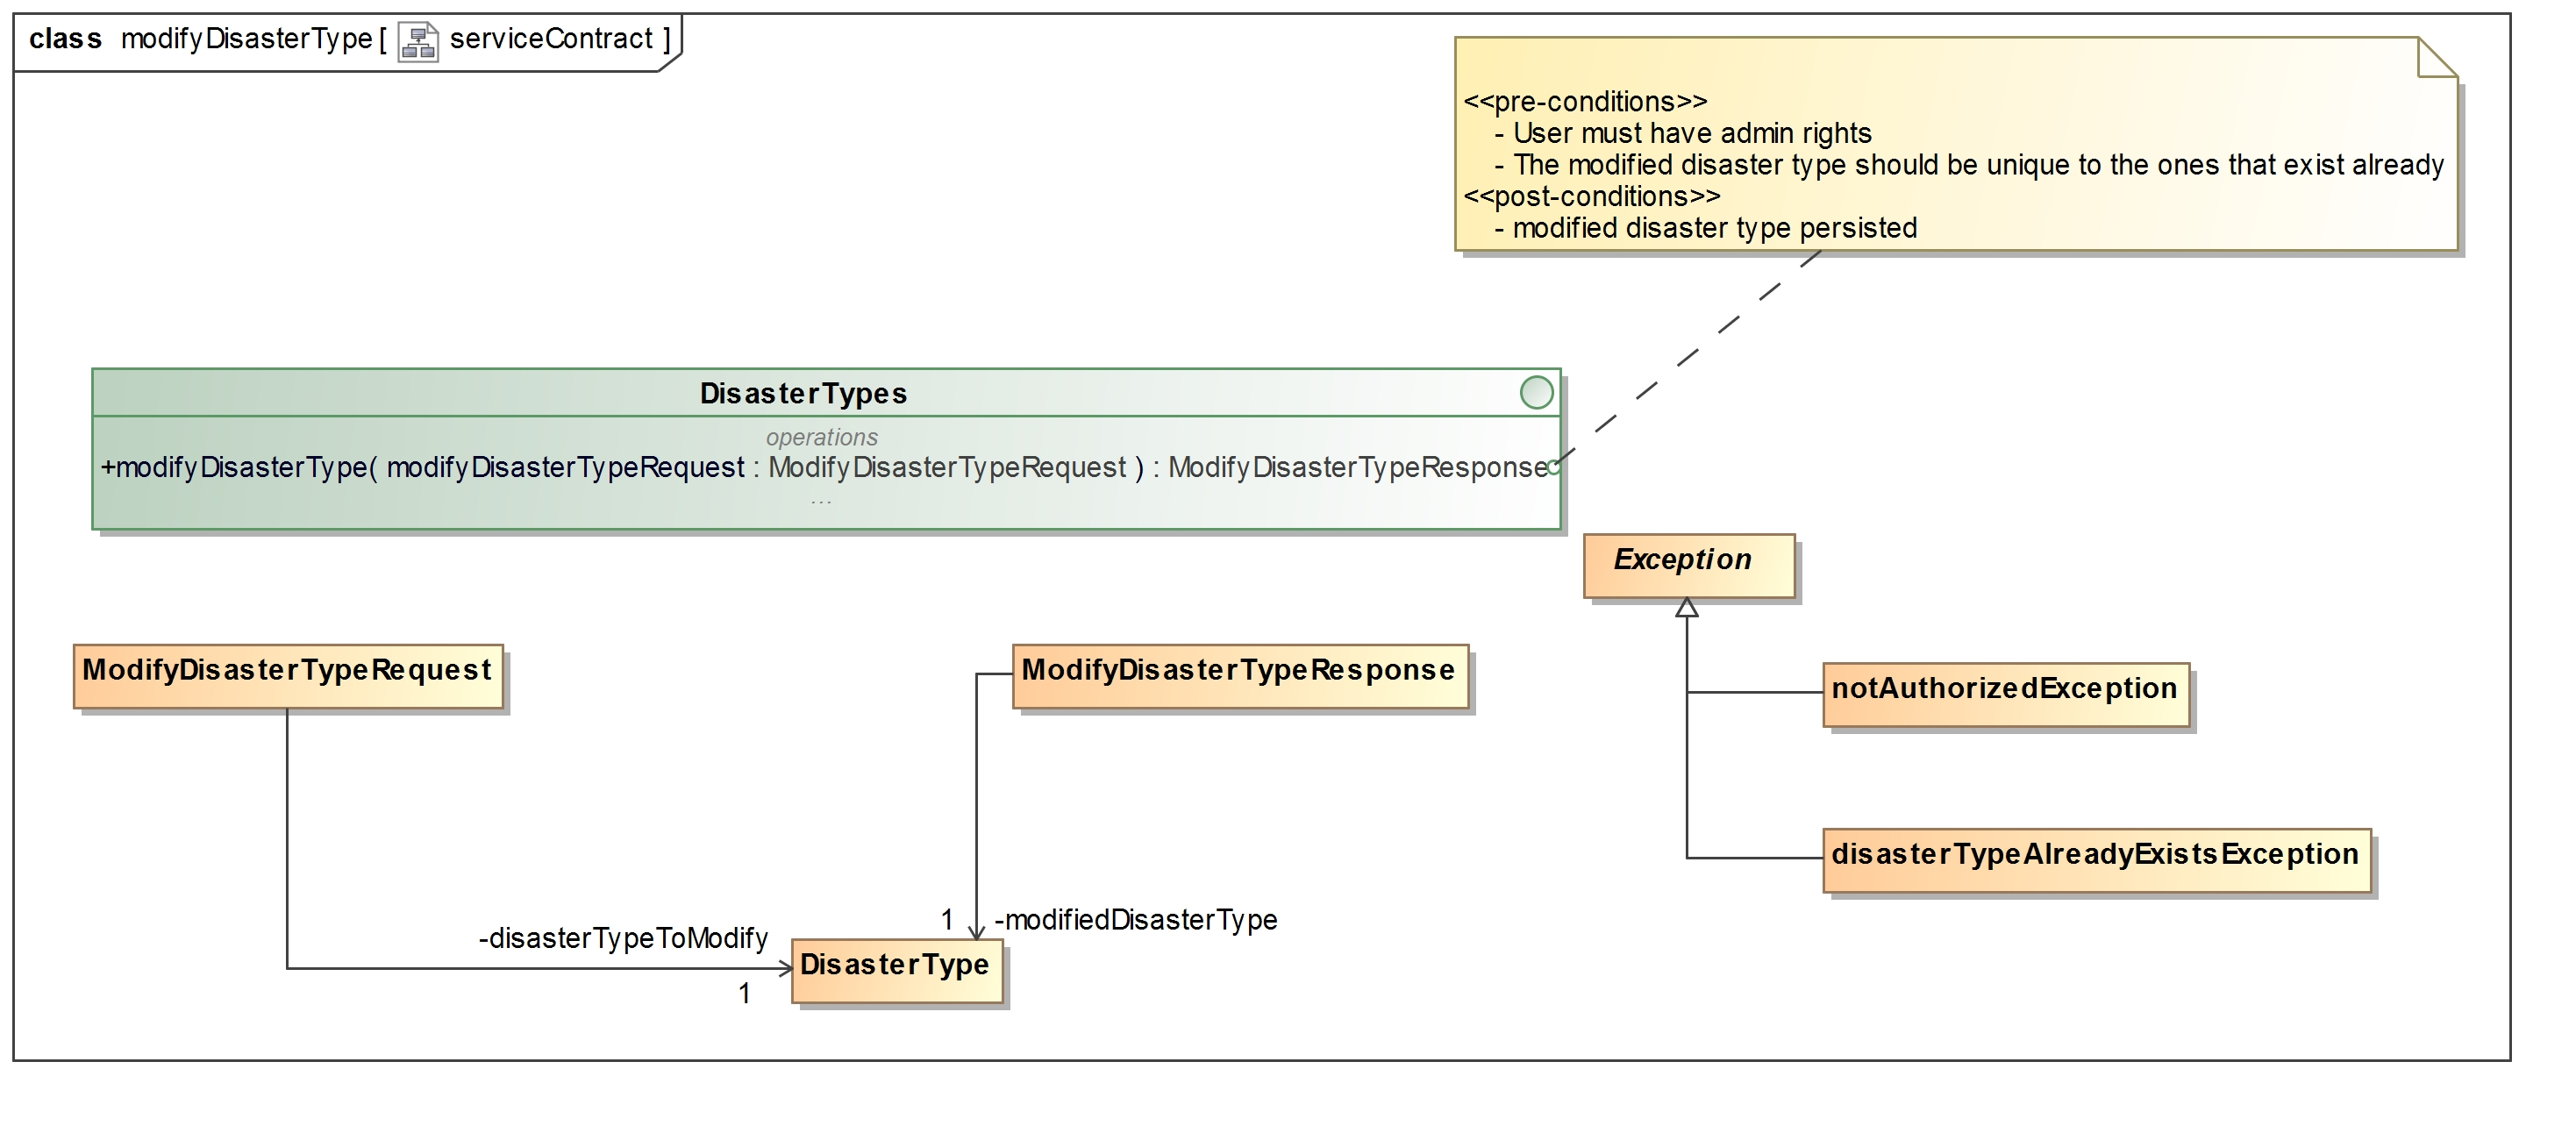
\includegraphics[scale=0.17]{../images/funcReq/modifyDisasterTypeServiceContract.jpg}
	\caption{The service contract for modifyDisasterType \label{overflow}}
\end{figure}

\begin{figure}[H]
	\centering
	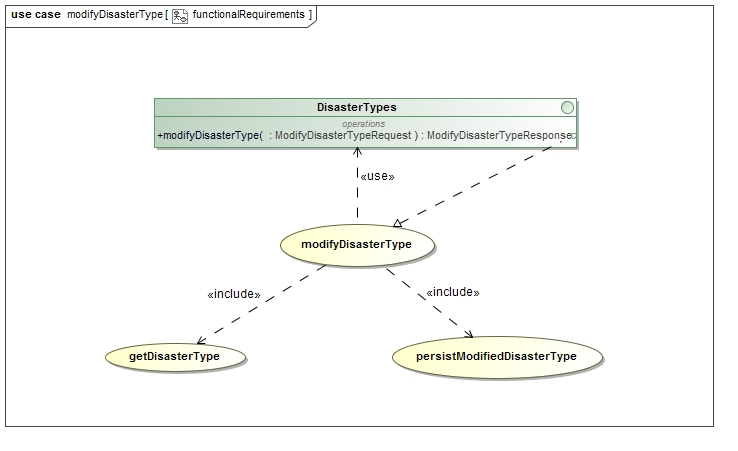
\includegraphics[width=1.2\textwidth]{../images/funcReq/modifyDisasterTypeFunctionalRequirements.jpg}
	\caption{The functional requirements diagram for modifyDisasterType \label{overflow}}
\end{figure}

\begin{figure}[H]
	\centering
	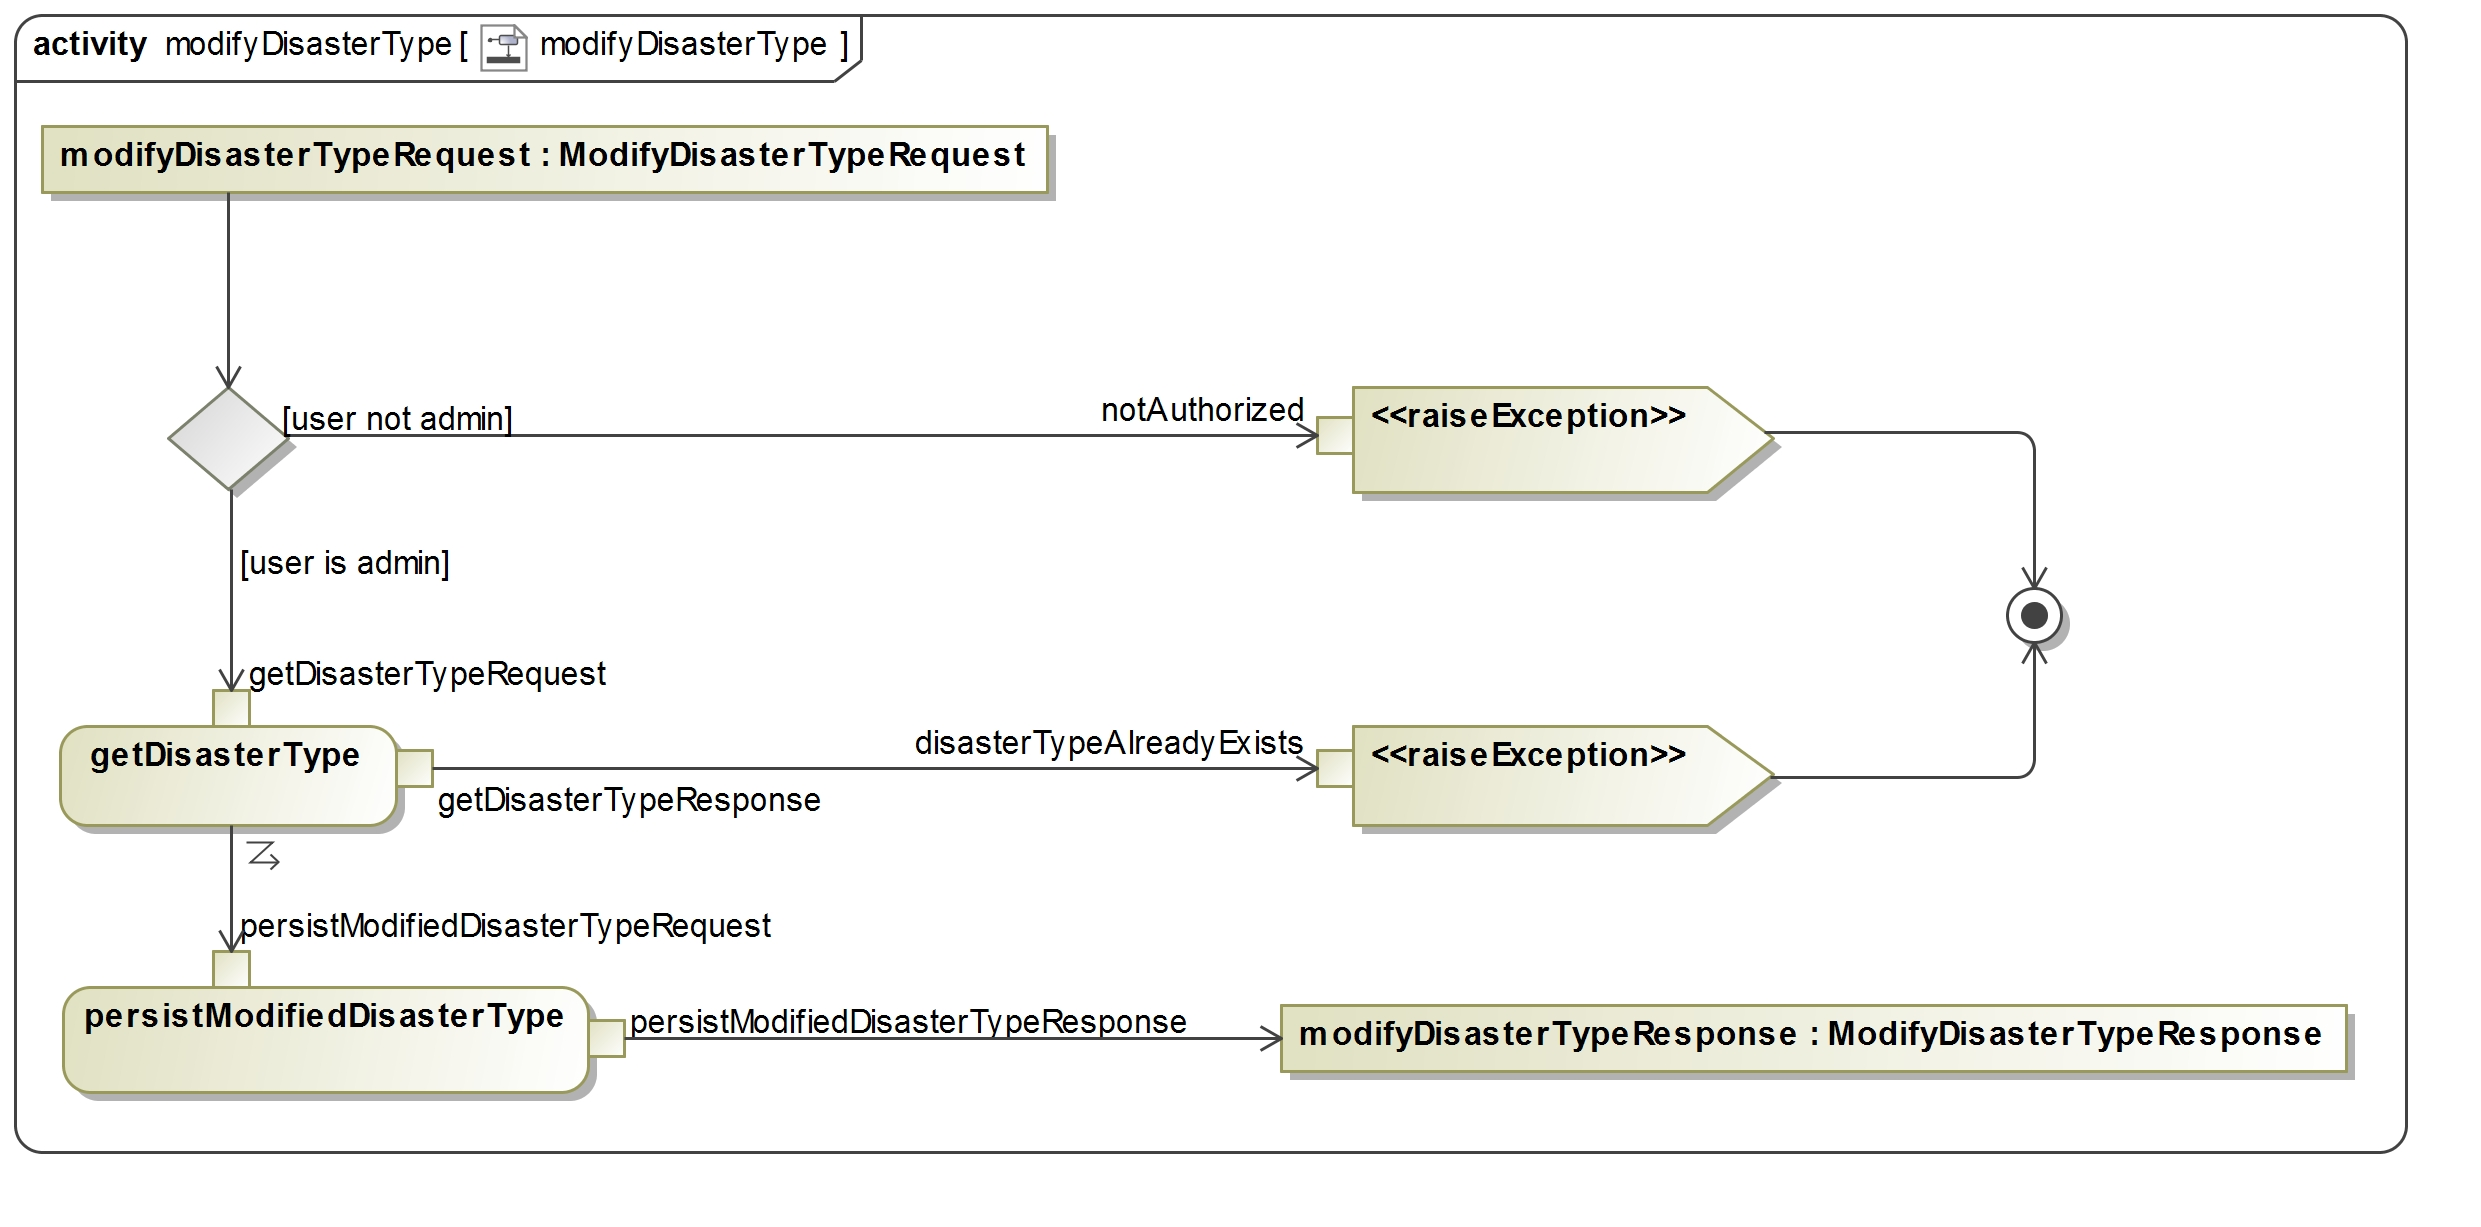
\includegraphics[scale=0.2]{../images/funcReq/modifyDisasterTypeActivityDiagram.jpg}
	\caption{The activity diagram for modifyDisasterType \label{overflow}}
\end{figure}